\documentclass[twoside]{book}

% Packages required by doxygen
\usepackage{fixltx2e}
\usepackage{calc}
\usepackage{doxygen}
\usepackage[export]{adjustbox} % also loads graphicx
\usepackage{graphicx}
\usepackage[utf8]{inputenc}
\usepackage{makeidx}
\usepackage{multicol}
\usepackage{multirow}
\PassOptionsToPackage{warn}{textcomp}
\usepackage{textcomp}
\usepackage[nointegrals]{wasysym}
\usepackage[table]{xcolor}

% NLS support packages
\usepackage[T2A]{fontenc}
\usepackage[russian]{babel}

% Font selection
\usepackage[T1]{fontenc}
\usepackage[scaled=.90]{helvet}
\usepackage{courier}
\usepackage{amssymb}
\usepackage{sectsty}
\renewcommand{\familydefault}{\sfdefault}
\allsectionsfont{%
  \fontseries{bc}\selectfont%
  \color{darkgray}%
}
\renewcommand{\DoxyLabelFont}{%
  \fontseries{bc}\selectfont%
  \color{darkgray}%
}
\newcommand{\+}{\discretionary{\mbox{\scriptsize$\hookleftarrow$}}{}{}}

% Page & text layout
\usepackage{geometry}
\geometry{%
  a4paper,%
  top=2.5cm,%
  bottom=2.5cm,%
  left=2.5cm,%
  right=2.5cm%
}
\tolerance=750
\hfuzz=15pt
\hbadness=750
\setlength{\emergencystretch}{15pt}
\setlength{\parindent}{0cm}
\setlength{\parskip}{3ex plus 2ex minus 2ex}
\makeatletter
\renewcommand{\paragraph}{%
  \@startsection{paragraph}{4}{0ex}{-1.0ex}{1.0ex}{%
    \normalfont\normalsize\bfseries\SS@parafont%
  }%
}
\renewcommand{\subparagraph}{%
  \@startsection{subparagraph}{5}{0ex}{-1.0ex}{1.0ex}{%
    \normalfont\normalsize\bfseries\SS@subparafont%
  }%
}
\makeatother

% Headers & footers
\usepackage{fancyhdr}
\pagestyle{fancyplain}
\fancyhead[LE]{\fancyplain{}{\bfseries\thepage}}
\fancyhead[CE]{\fancyplain{}{}}
\fancyhead[RE]{\fancyplain{}{\bfseries\leftmark}}
\fancyhead[LO]{\fancyplain{}{\bfseries\rightmark}}
\fancyhead[CO]{\fancyplain{}{}}
\fancyhead[RO]{\fancyplain{}{\bfseries\thepage}}
\fancyfoot[LE]{\fancyplain{}{}}
\fancyfoot[CE]{\fancyplain{}{}}
\fancyfoot[RE]{\fancyplain{}{\bfseries\scriptsize Создано системой Doxygen }}
\fancyfoot[LO]{\fancyplain{}{\bfseries\scriptsize Создано системой Doxygen }}
\fancyfoot[CO]{\fancyplain{}{}}
\fancyfoot[RO]{\fancyplain{}{}}
\renewcommand{\footrulewidth}{0.4pt}
\renewcommand{\chaptermark}[1]{%
  \markboth{#1}{}%
}
\renewcommand{\sectionmark}[1]{%
  \markright{\thesection\ #1}%
}

% Indices & bibliography
\usepackage{natbib}
\usepackage[titles]{tocloft}
\setcounter{tocdepth}{3}
\setcounter{secnumdepth}{5}
\makeindex

% Hyperlinks (required, but should be loaded last)
\usepackage{ifpdf}
\ifpdf
  \usepackage[pdftex,pagebackref=true]{hyperref}
\else
  \usepackage[ps2pdf,pagebackref=true]{hyperref}
\fi
\hypersetup{%
  colorlinks=true,%
  linkcolor=blue,%
  citecolor=blue,%
  unicode%
}

% Custom commands
\newcommand{\clearemptydoublepage}{%
  \newpage{\pagestyle{empty}\cleardoublepage}%
}

\usepackage{caption}
\captionsetup{labelsep=space,justification=centering,font={bf},singlelinecheck=off,skip=4pt,position=top}

%===== C O N T E N T S =====

\begin{document}

% Titlepage & ToC
\hypersetup{pageanchor=false,
             bookmarksnumbered=true,
             pdfencoding=unicode
            }
\pagenumbering{alph}
\begin{titlepage}
\vspace*{7cm}
\begin{center}%
{\Large Permutation cipher \\[1ex]\large 1.\+0.\+0 }\\
\vspace*{1cm}
{\large Создано системой Doxygen 1.8.13}\\
\end{center}
\end{titlepage}
\clearemptydoublepage
\pagenumbering{roman}
\tableofcontents
\clearemptydoublepage
\pagenumbering{arabic}
\hypersetup{pageanchor=true}

%--- Begin generated contents ---
\chapter{Иерархический список классов}
\section{Иерархия классов}
Иерархия классов.\begin{DoxyCompactList}
\item \contentsline{section}{Cipher}{\pageref{classCipher}}{}
\item invalid\+\_\+argument\begin{DoxyCompactList}
\item \contentsline{section}{cipher\+\_\+error}{\pageref{classcipher__error}}{}
\end{DoxyCompactList}
\end{DoxyCompactList}

\chapter{Алфавитный указатель классов}
\section{Классы}
Классы с их кратким описанием.\begin{DoxyCompactList}
\item\contentsline{section}{\hyperlink{classCipher}{Cipher} \\*Шифрование методом табличной перестановки }{\pageref{classCipher}}{}
\item\contentsline{section}{\hyperlink{classcipher__error}{cipher\+\_\+error} \\*Класс-\/исключение }{\pageref{classcipher__error}}{}
\end{DoxyCompactList}

\chapter{Список файлов}
\section{Файлы}
Полный список документированных файлов.\begin{DoxyCompactList}
\item\contentsline{section}{\hyperlink{Cipher_8h}{Cipher.\+h} \\*Класс-\/исключение }{\pageref{Cipher_8h}}{}
\end{DoxyCompactList}

\chapter{Классы}
\hypertarget{classCipher}{}\section{Класс Cipher}
\label{classCipher}\index{Cipher@{Cipher}}


Шифрование методом табличной перестановки  




{\ttfamily \#include $<$Cipher.\+h$>$}

\subsection*{Открытые члены}
\begin{DoxyCompactItemize}
\item 
\mbox{\Hypertarget{classCipher_ae728d0917db639dd49638a268298391f}\label{classCipher_ae728d0917db639dd49638a268298391f}} 
\hyperlink{classCipher_ae728d0917db639dd49638a268298391f}{Cipher} ()=delete
\begin{DoxyCompactList}\small\item\em Конструктор по умолчанию запрещён \end{DoxyCompactList}\item 
\hyperlink{classCipher_a876edcc7064f450935baedce442f1556}{Cipher} (std\+::wstring \&ws\+\_\+key)
\begin{DoxyCompactList}\small\item\em Конструктор принимает ключ (количество столбцов в таблице) \end{DoxyCompactList}\item 
std\+::wstring \hyperlink{classCipher_aebf6146bc7bb26d9b934ced49ed6dd19}{encrypt} (std\+::wstring \&ws\+\_\+open\+\_\+text)
\begin{DoxyCompactList}\small\item\em Метод для зашифрования \end{DoxyCompactList}\item 
std\+::wstring \hyperlink{classCipher_accb629416e343719818e557b8eb994dd}{decrypt} (const std\+::wstring \&ws\+\_\+cipher\+\_\+text)
\begin{DoxyCompactList}\small\item\em Метод для расшифрования \end{DoxyCompactList}\item 
void \hyperlink{classCipher_ae40ca9f1c13890b6d734aa9228d0de28}{set\+\_\+tableform} (const std\+::wstring \&ws\+\_\+text)
\begin{DoxyCompactList}\small\item\em Формирование информации о таблице \end{DoxyCompactList}\item 
void \hyperlink{classCipher_a86145f7c206e6d75852a28ffe29dc47a}{set\+\_\+key} (std\+::wstring \&ws\+\_\+key)
\begin{DoxyCompactList}\small\item\em Установка нового ключа \end{DoxyCompactList}\item 
int \hyperlink{classCipher_aec5962319726c6dd1bd6ee2f7b71e001}{get\+Valid\+Key} (std\+::wstring \&ws\+\_\+key)
\begin{DoxyCompactList}\small\item\em Проверка на правильность ключа \end{DoxyCompactList}\item 
std\+::wstring \hyperlink{classCipher_a0dc9d7c13d6a7401bfee1f1171f6ee12}{get\+Valid\+Open\+Text} (const std\+::wstring \&ws\+\_\+open\+\_\+text)
\begin{DoxyCompactList}\small\item\em Проверка на правильность текста для зашифровки \end{DoxyCompactList}\item 
std\+::wstring \hyperlink{classCipher_ab0e1d86022b18c1bec07cde229ba87e6}{get\+Valid\+Cipher\+Text} (const std\+::wstring \&ws\+\_\+cipher\+\_\+text)
\begin{DoxyCompactList}\small\item\em Проверка на правильность текста для расшифровки \end{DoxyCompactList}\end{DoxyCompactItemize}
\subsection*{Закрытые данные}
\begin{DoxyCompactItemize}
\item 
\mbox{\Hypertarget{classCipher_a771e84ee997948183d065a2804f3cda6}\label{classCipher_a771e84ee997948183d065a2804f3cda6}} 
std\+::wstring\+\_\+convert$<$ std\+::codecvt\+\_\+utf8$<$ wchar\+\_\+t $>$, wchar\+\_\+t $>$ \hyperlink{classCipher_a771e84ee997948183d065a2804f3cda6}{codec}
\begin{DoxyCompactList}\small\item\em codec для преобразования в широкий формат строки и обратно \end{DoxyCompactList}\item 
\mbox{\Hypertarget{classCipher_a4fa1fd596bd312cbf0f7628ac72a60d5}\label{classCipher_a4fa1fd596bd312cbf0f7628ac72a60d5}} 
int \hyperlink{classCipher_a4fa1fd596bd312cbf0f7628ac72a60d5}{columns}
\begin{DoxyCompactList}\small\item\em Количество столбцов в таблице (ключ) \end{DoxyCompactList}\item 
\mbox{\Hypertarget{classCipher_ace25b12087068c25c945e2a32a236f9e}\label{classCipher_ace25b12087068c25c945e2a32a236f9e}} 
int \hyperlink{classCipher_ace25b12087068c25c945e2a32a236f9e}{rows}
\begin{DoxyCompactList}\small\item\em Количество строк в таблице \end{DoxyCompactList}\item 
\mbox{\Hypertarget{classCipher_a84f8e0da2b41787fa92554549963f052}\label{classCipher_a84f8e0da2b41787fa92554549963f052}} 
int \hyperlink{classCipher_a84f8e0da2b41787fa92554549963f052}{len\+\_\+text}
\begin{DoxyCompactList}\small\item\em Количество символов в слове \end{DoxyCompactList}\end{DoxyCompactItemize}


\subsection{Подробное описание}
Шифрование методом табличной перестановки 

Ключ устанавливается в конструкторе, а также с помощью метода set\+\_\+key. Для зашифрования и расшифрования предназначены методы encrypt и decrypt. Метод set\+\_\+tableform -\/ вспомогающий. Методы\+: get\+Valid\+Key, get\+Valid\+Open\+Text, get\+Valid\+Cipher\+Text -\/ специализируются на проверке входных данных. \begin{DoxyWarning}{Предупреждения}
Реализация только для русского языка! С использованием wstring.\+Шифрование методом табличной перестановки 
\end{DoxyWarning}


\subsection{Конструктор(ы)}
\mbox{\Hypertarget{classCipher_a876edcc7064f450935baedce442f1556}\label{classCipher_a876edcc7064f450935baedce442f1556}} 
\index{Cipher@{Cipher}!Cipher@{Cipher}}
\index{Cipher@{Cipher}!Cipher@{Cipher}}
\subsubsection{\texorpdfstring{Cipher()}{Cipher()}}
{\footnotesize\ttfamily Cipher\+::\+Cipher (\begin{DoxyParamCaption}\item[{std\+::wstring \&}]{ws\+\_\+key }\end{DoxyParamCaption})}



Конструктор принимает ключ (количество столбцов в таблице) 

Конструктор, принимающий на вход ключ, устанавливает кол-\/во столбцов


\begin{DoxyParams}{Аргументы}
{\em ws\+\_\+key} & \\
\hline
\end{DoxyParams}
\begin{DoxyReturn}{Возвращает}
Ничего не возвращает 
\end{DoxyReturn}


\subsection{Методы}
\mbox{\Hypertarget{classCipher_accb629416e343719818e557b8eb994dd}\label{classCipher_accb629416e343719818e557b8eb994dd}} 
\index{Cipher@{Cipher}!decrypt@{decrypt}}
\index{decrypt@{decrypt}!Cipher@{Cipher}}
\subsubsection{\texorpdfstring{decrypt()}{decrypt()}}
{\footnotesize\ttfamily std\+::wstring Cipher\+::decrypt (\begin{DoxyParamCaption}\item[{const std\+::wstring \&}]{cipher\+\_\+text }\end{DoxyParamCaption})}



Метод для расшифрования 

Метод decrypt расшифровывает текст.


\begin{DoxyParams}{Аргументы}
{\em cipher\+\_\+text} & \\
\hline
\end{DoxyParams}
\begin{DoxyReturn}{Возвращает}
Зашифрованный текст. 
\end{DoxyReturn}
\mbox{\Hypertarget{classCipher_aebf6146bc7bb26d9b934ced49ed6dd19}\label{classCipher_aebf6146bc7bb26d9b934ced49ed6dd19}} 
\index{Cipher@{Cipher}!encrypt@{encrypt}}
\index{encrypt@{encrypt}!Cipher@{Cipher}}
\subsubsection{\texorpdfstring{encrypt()}{encrypt()}}
{\footnotesize\ttfamily std\+::wstring Cipher\+::encrypt (\begin{DoxyParamCaption}\item[{std\+::wstring \&}]{open\+\_\+text }\end{DoxyParamCaption})}



Метод для зашифрования 

Метод encrypt зашифровывает текст.


\begin{DoxyParams}{Аргументы}
{\em open\+\_\+text} & \\
\hline
\end{DoxyParams}
\begin{DoxyReturn}{Возвращает}
Зашифрованный текст 
\end{DoxyReturn}
\mbox{\Hypertarget{classCipher_ab0e1d86022b18c1bec07cde229ba87e6}\label{classCipher_ab0e1d86022b18c1bec07cde229ba87e6}} 
\index{Cipher@{Cipher}!get\+Valid\+Cipher\+Text@{get\+Valid\+Cipher\+Text}}
\index{get\+Valid\+Cipher\+Text@{get\+Valid\+Cipher\+Text}!Cipher@{Cipher}}
\subsubsection{\texorpdfstring{get\+Valid\+Cipher\+Text()}{getValidCipherText()}}
{\footnotesize\ttfamily std\+::wstring Cipher\+::get\+Valid\+Cipher\+Text (\begin{DoxyParamCaption}\item[{const std\+::wstring \&}]{ws\+\_\+cipher\+\_\+text }\end{DoxyParamCaption})\hspace{0.3cm}{\ttfamily [inline]}}



Проверка на правильность текста для расшифровки 

Данный метод проверяет зашифрованный текст на правильность.


\begin{DoxyParams}{Аргументы}
{\em ws\+\_\+cipher\+\_\+text} & \\
\hline
\end{DoxyParams}
\begin{DoxyReturn}{Возвращает}
Зашифрованный текст 
\end{DoxyReturn}

\begin{DoxyExceptions}{Исключения}
{\em \hyperlink{classcipher__error}{cipher\+\_\+error},если} & текст пустой или невалидный \\
\hline
\end{DoxyExceptions}
\mbox{\Hypertarget{classCipher_aec5962319726c6dd1bd6ee2f7b71e001}\label{classCipher_aec5962319726c6dd1bd6ee2f7b71e001}} 
\index{Cipher@{Cipher}!get\+Valid\+Key@{get\+Valid\+Key}}
\index{get\+Valid\+Key@{get\+Valid\+Key}!Cipher@{Cipher}}
\subsubsection{\texorpdfstring{get\+Valid\+Key()}{getValidKey()}}
{\footnotesize\ttfamily int Cipher\+::get\+Valid\+Key (\begin{DoxyParamCaption}\item[{std\+::wstring \&}]{ws\+\_\+key }\end{DoxyParamCaption})\hspace{0.3cm}{\ttfamily [inline]}}



Проверка на правильность ключа 

Данный метод проверяет ключ на правильность.


\begin{DoxyParams}{Аргументы}
{\em ws\+\_\+key} & \\
\hline
\end{DoxyParams}
\begin{DoxyReturn}{Возвращает}
Ключ 
\end{DoxyReturn}

\begin{DoxyExceptions}{Исключения}
{\em \hyperlink{classcipher__error}{cipher\+\_\+error},если} & ключ пустой или невалидный \\
\hline
\end{DoxyExceptions}
\mbox{\Hypertarget{classCipher_a0dc9d7c13d6a7401bfee1f1171f6ee12}\label{classCipher_a0dc9d7c13d6a7401bfee1f1171f6ee12}} 
\index{Cipher@{Cipher}!get\+Valid\+Open\+Text@{get\+Valid\+Open\+Text}}
\index{get\+Valid\+Open\+Text@{get\+Valid\+Open\+Text}!Cipher@{Cipher}}
\subsubsection{\texorpdfstring{get\+Valid\+Open\+Text()}{getValidOpenText()}}
{\footnotesize\ttfamily std\+::wstring Cipher\+::get\+Valid\+Open\+Text (\begin{DoxyParamCaption}\item[{const std\+::wstring \&}]{ws\+\_\+open\+\_\+text }\end{DoxyParamCaption})\hspace{0.3cm}{\ttfamily [inline]}}



Проверка на правильность текста для зашифровки 

Данный метод проверяет открытый текст на правильность. Строчные буквы превращаются в прописные. Все не-\/буквы удаляются.


\begin{DoxyParams}{Аргументы}
{\em ws\+\_\+open\+\_\+text} & \\
\hline
\end{DoxyParams}
\begin{DoxyReturn}{Возвращает}
Текст для расшифровки 
\end{DoxyReturn}

\begin{DoxyExceptions}{Исключения}
{\em \hyperlink{classcipher__error}{cipher\+\_\+error},если} & текст пустой \\
\hline
\end{DoxyExceptions}
\mbox{\Hypertarget{classCipher_a86145f7c206e6d75852a28ffe29dc47a}\label{classCipher_a86145f7c206e6d75852a28ffe29dc47a}} 
\index{Cipher@{Cipher}!set\+\_\+key@{set\+\_\+key}}
\index{set\+\_\+key@{set\+\_\+key}!Cipher@{Cipher}}
\subsubsection{\texorpdfstring{set\+\_\+key()}{set\_key()}}
{\footnotesize\ttfamily void Cipher\+::set\+\_\+key (\begin{DoxyParamCaption}\item[{std\+::wstring \&}]{ws\+\_\+key }\end{DoxyParamCaption})}



Установка нового ключа 

Метод, принимающий на вход ключ, устанавливает кол-\/во столбцов


\begin{DoxyParams}{Аргументы}
{\em ws\+\_\+key} & \\
\hline
\end{DoxyParams}
\begin{DoxyReturn}{Возвращает}
Ничего не возвращает 
\end{DoxyReturn}
\mbox{\Hypertarget{classCipher_ae40ca9f1c13890b6d734aa9228d0de28}\label{classCipher_ae40ca9f1c13890b6d734aa9228d0de28}} 
\index{Cipher@{Cipher}!set\+\_\+tableform@{set\+\_\+tableform}}
\index{set\+\_\+tableform@{set\+\_\+tableform}!Cipher@{Cipher}}
\subsubsection{\texorpdfstring{set\+\_\+tableform()}{set\_tableform()}}
{\footnotesize\ttfamily void Cipher\+::set\+\_\+tableform (\begin{DoxyParamCaption}\item[{const std\+::wstring \&}]{open\+\_\+text }\end{DoxyParamCaption})}



Формирование информации о таблице 

Принимает текст для зашифровки, далее по нему формирует кол-\/во строк в таблице, а также получает длину текста.


\begin{DoxyParams}{Аргументы}
{\em open\+\_\+text} & \\
\hline
\end{DoxyParams}


Объявления и описания членов классов находятся в файлах\+:\begin{DoxyCompactItemize}
\item 
\hyperlink{Cipher_8h}{Cipher.\+h}\item 
Cipher.\+cpp\end{DoxyCompactItemize}

\hypertarget{classcipher__error}{}\section{Класс cipher\+\_\+error}
\label{classcipher__error}\index{cipher\+\_\+error@{cipher\+\_\+error}}


Класс-\/исключение  




{\ttfamily \#include $<$Cipher.\+h$>$}



Граф наследования\+:cipher\+\_\+error\+:
\nopagebreak
\begin{figure}[H]
\begin{center}
\leavevmode
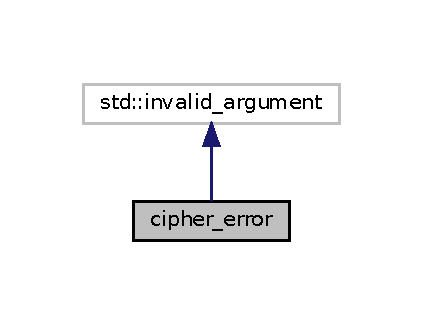
\includegraphics[width=203pt]{classcipher__error__inherit__graph}
\end{center}
\end{figure}


Граф связей класса cipher\+\_\+error\+:
\nopagebreak
\begin{figure}[H]
\begin{center}
\leavevmode
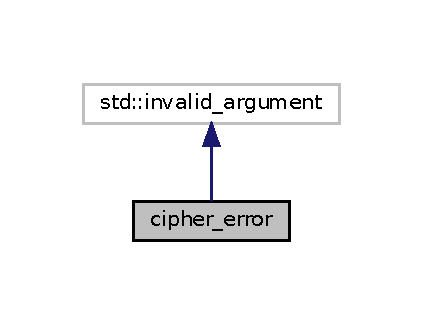
\includegraphics[width=203pt]{classcipher__error__coll__graph}
\end{center}
\end{figure}
\subsection*{Открытые члены}
\begin{DoxyCompactItemize}
\item 
\hyperlink{classcipher__error_aac662e216a84bfeb873303c7b88d029e}{cipher\+\_\+error} (const std\+::string \&what\+\_\+arg)
\begin{DoxyCompactList}\small\item\em Принимает строку, поднимает исключение \end{DoxyCompactList}\item 
\hyperlink{classcipher__error_a18cf27d9c2cd2538d3cb8f17e9a55f3e}{cipher\+\_\+error} (const char $\ast$what\+\_\+arg)
\begin{DoxyCompactList}\small\item\em Принимает си строку, поднимает исключение \end{DoxyCompactList}\end{DoxyCompactItemize}


\subsection{Подробное описание}
Класс-\/исключение 

\subsection{Конструктор(ы)}
\mbox{\Hypertarget{classcipher__error_aac662e216a84bfeb873303c7b88d029e}\label{classcipher__error_aac662e216a84bfeb873303c7b88d029e}} 
\index{cipher\+\_\+error@{cipher\+\_\+error}!cipher\+\_\+error@{cipher\+\_\+error}}
\index{cipher\+\_\+error@{cipher\+\_\+error}!cipher\+\_\+error@{cipher\+\_\+error}}
\subsubsection{\texorpdfstring{cipher\+\_\+error()}{cipher\_error()}\hspace{0.1cm}{\footnotesize\ttfamily [1/2]}}
{\footnotesize\ttfamily cipher\+\_\+error\+::cipher\+\_\+error (\begin{DoxyParamCaption}\item[{const std\+::string \&}]{what\+\_\+arg }\end{DoxyParamCaption})\hspace{0.3cm}{\ttfamily [inline]}, {\ttfamily [explicit]}}



Принимает строку, поднимает исключение 


\begin{DoxyParams}{Аргументы}
{\em what\+\_\+arg} & \\
\hline
\end{DoxyParams}
\mbox{\Hypertarget{classcipher__error_a18cf27d9c2cd2538d3cb8f17e9a55f3e}\label{classcipher__error_a18cf27d9c2cd2538d3cb8f17e9a55f3e}} 
\index{cipher\+\_\+error@{cipher\+\_\+error}!cipher\+\_\+error@{cipher\+\_\+error}}
\index{cipher\+\_\+error@{cipher\+\_\+error}!cipher\+\_\+error@{cipher\+\_\+error}}
\subsubsection{\texorpdfstring{cipher\+\_\+error()}{cipher\_error()}\hspace{0.1cm}{\footnotesize\ttfamily [2/2]}}
{\footnotesize\ttfamily cipher\+\_\+error\+::cipher\+\_\+error (\begin{DoxyParamCaption}\item[{const char $\ast$}]{what\+\_\+arg }\end{DoxyParamCaption})\hspace{0.3cm}{\ttfamily [inline]}, {\ttfamily [explicit]}}



Принимает си строку, поднимает исключение 


\begin{DoxyParams}{Аргументы}
{\em what\+\_\+arg} & \\
\hline
\end{DoxyParams}


Объявления и описания членов класса находятся в файле\+:\begin{DoxyCompactItemize}
\item 
\hyperlink{Cipher_8h}{Cipher.\+h}\end{DoxyCompactItemize}

\chapter{Файлы}
\hypertarget{Cipher_8h}{}\section{Файл Cipher.\+h}
\label{Cipher_8h}\index{Cipher.\+h@{Cipher.\+h}}


Класс-\/исключение  


{\ttfamily \#include $<$vector$>$}\newline
{\ttfamily \#include $<$string$>$}\newline
{\ttfamily \#include $<$map$>$}\newline
{\ttfamily \#include $<$codecvt$>$}\newline
{\ttfamily \#include $<$locale$>$}\newline
{\ttfamily \#include $<$iostream$>$}\newline
Граф включаемых заголовочных файлов для Cipher.\+h\+:
\nopagebreak
\begin{figure}[H]
\begin{center}
\leavevmode
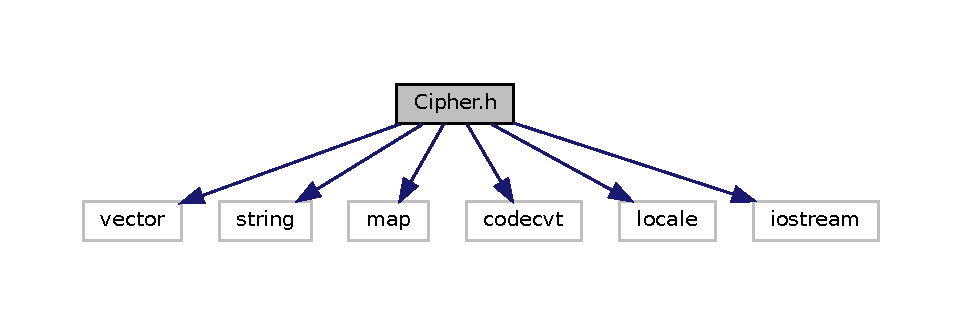
\includegraphics[width=350pt]{Cipher_8h__incl}
\end{center}
\end{figure}
\subsection*{Классы}
\begin{DoxyCompactItemize}
\item 
class \hyperlink{classCipher}{Cipher}
\begin{DoxyCompactList}\small\item\em Шифрование методом табличной перестановки \end{DoxyCompactList}\item 
class \hyperlink{classcipher__error}{cipher\+\_\+error}
\begin{DoxyCompactList}\small\item\em Класс-\/исключение \end{DoxyCompactList}\end{DoxyCompactItemize}


\subsection{Подробное описание}
Класс-\/исключение 


%--- End generated contents ---

% Index
\backmatter
\newpage
\phantomsection
\clearemptydoublepage
\addcontentsline{toc}{chapter}{Алфавитный указатель}
\printindex

\end{document}
